\documentclass[10pt,pdf,utf8,russian,aspectratio=169]{beamer}
\usepackage[T2A]{fontenc}
\usetheme{Singapore}
\usepackage{setspace}
\usepackage{amsmath}
\usepackage{pgfplots}
\usepackage[utf8]{inputenc}
\usepackage{tikz-cd}
\usepackage[all, 2cell]{xy}
\usepackage{amssymb}
\usepackage{verba tim}
\usepackage[all]{xy}
\usepackage{tikz}
\usepackage{bussproofs}
\usepackage{dsfont}
\usepackage{mathabx}
\usepackage{animate}
\usetikzlibrary{graphs}
\usetikzlibrary{arrows}
\usepackage{hyperref}
\usepackage[english,russian]{babel}
\usepackage{listings}
\usepackage{color}
\usepackage{tikz}
\usepackage{listings}
\pgfplotsset{compat=1.16}
\newtheorem{defin}{Definition}
\newtheorem{theor}{Theorem}
\newtheorem{prop}{Proposition}
\title{Functional programming, Seminar No. 3}
\author{Danya Rogozin \\ Lomonosov Moscow State University, \\ Serokell O\"{U}}
\date{Higher School of Economics \\ Faculty of Computer Science}
\begin{document}
\lstset{
  frame=none,
  xleftmargin=2pt,
  stepnumber=1,
  numbers=left,
  numbersep=5pt,
  numberstyle=\ttfamily\tiny\color[gray]{0.3},
  belowcaptionskip=\bigskipamount,
  captionpos=b,
  escapeinside={*'}{'*},
  language=haskell,
  tabsize=2,
  emphstyle={\bf},
  commentstyle=\it,
  stringstyle=\mdseries\rmfamily,
  showspaces=false,
  keywordstyle=\bfseries\rmfamily,
  columns=flexible,
  basicstyle=\small\sffamily,
  showstringspaces=false,
  morecomment=[l]\%,
}
\maketitle

\begin{frame}
  \frametitle{Intro}

  On the previous seminar, we
  \onslide<1->{
  \begin{itemize}
    \item studied the basic Haskell syntax
    \item introduced the notion of a weak head normal form to describe the operatonal semantics of Haskell
    \item analysed the regrettable cicrumstances according to which Haskell doesn't have the Church-Rosser property as a system of typed lambda calculus
  \end{itemize}
  }

\vspace{\baselineskip}

\onslide<2->{
Today we
  \begin{itemize}
    \item investigate the Haskell type system more deeply and overview the advantages of parametric polymorphism
    \item take a look at bounded polymorphism and discuss type classes
  \end{itemize}
  }
\end{frame}

\begin{frame}[fragile]
  \frametitle{Motivation}
  Let us recall the example of a higher order function from the previous seminar:

  \begin{lstlisting}[language=Haskell]
  changeTwiceBy :: (Int -> Int) -> Int -> Int
  changeTwiceBy operation value = operation (operation value)
  \end{lstlisting}

  \vspace{\baselineskip}

  It is clear that one may implement the function for Boolean values and strings that have the same behaviour as the function above:

  \begin{lstlisting}[language=Haskell]
  changeTwiceByBool :: (Bool -> Bool) -> Bool -> Bool
  changeTwiceByBool operation value = operation (operation value)

  changeTwiceByString :: (String -> String) -> String -> String
  changeTwiceByString operation value = operation (operation value)
  \end{lstlisting}

  \onslide<2->{
  One needs to have a way to avoid such a boilerplate.
  }
\end{frame}

\begin{frame}[fragile]
  \frametitle{Parametric polymorphism}

The key idea of parametric polymorphism that the same function might be called on distinct data types. Here are the first polymorphic examples:

  \begin{lstlisting}[language=Haskell]
  id :: a -> a
  id x = x

  const :: a -> b -> a
  const a b = a

  fst :: (a, b) -> a
  fst (a, b) = a

  snd :: (a, b) -> b
  snd = "guess what"

  swap :: (a, b) -> (b, a)
  swap (a, b) = (b, a)
  \end{lstlisting}
\end{frame}

\begin{frame}
  \frametitle{The meme time}

  \begin{center}
  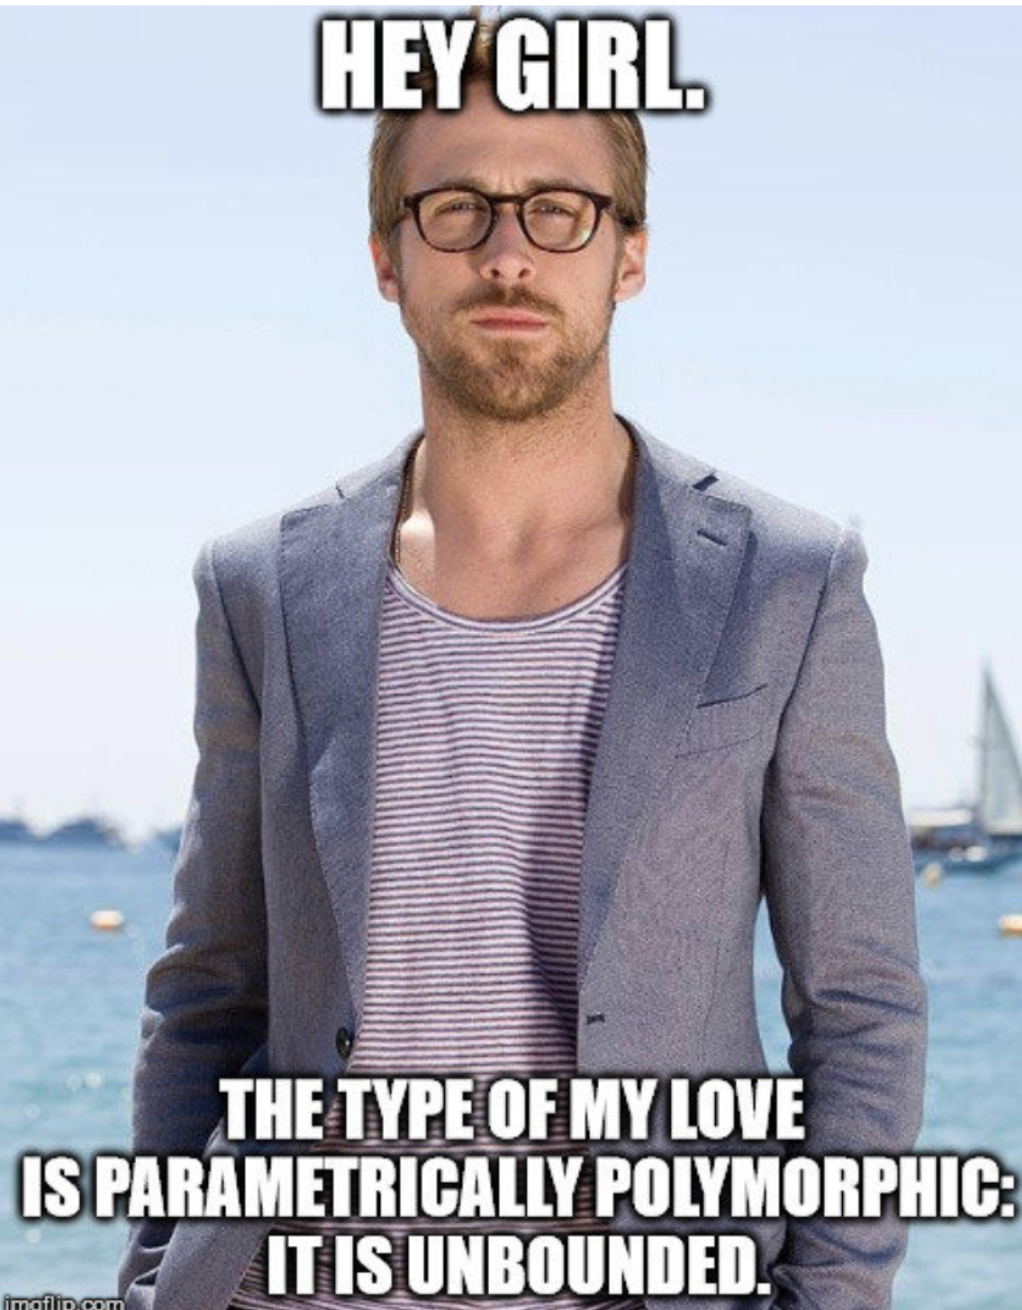
\includegraphics[scale=0.3]{Pics/Ryan.png}
  \end{center}
\end{frame}

\begin{frame}
  \frametitle{The functions above in the GHCi session}

  \begin{center}
  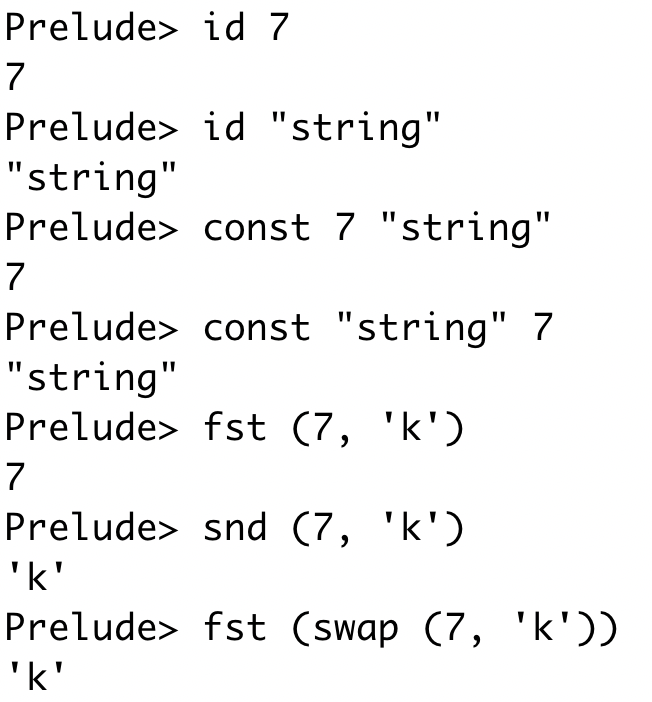
\includegraphics[scale=0.5]{Pics/Triv.png}
  \end{center}
\end{frame}

\begin{frame}[fragile]
  \frametitle{A brief clarification}

\begin{itemize}
  \item In such signatures as $a \to b \to a$, $a, b$ are type variables that range over arbitrary data types. In fact, $a$, $b$ are bounded by universal quantifier that hidden under the carpet.
  \item In a matter of fact, the functions from the previous slide have the following signatures:
  \begin{lstlisting}[language=Haskell]
  id :: forall a. a -> a
  id x = x

  const :: forall a b. a -> b -> a
  const a b = a

  fst :: forall a b. (a, b) -> a
  fst (a, b) = a

  swap :: forall a b. (a, b) -> (b, a)
  swap (a, b) = (b, a)
  \end{lstlisting}
\end{itemize}
\end{frame}

\begin{frame}[fragile]
  \frametitle{Higher order functions and parametric polymorpism}

  \begin{lstlisting}[language=Haskell]
  infixr 9 .
  (.) :: (b -> c) -> (a -> b) -> a -> c
  f . g = \x -> f (g x)

  flip :: (a -> b -> c) -> b -> a -> c
  flip f b a = f a b

  fix :: (a -> a) -> a
  fix f = f (fix f)

  curry :: ((a, b) -> c) -> a -> b -> c
  curry f x y = f (x, y)

  uncurry :: (a -> b -> c) -> ((a, b) -> c)
  uncurry f p = f (fst p) (snd p)
  \end{lstlisting}
\end{frame}

\begin{frame}[fragile]
    \frametitle{The functions above in the GHCi session. The composition examples}

\begin{lstlisting}[language=Haskell]
incNegate :: Int -> Int
incNegate x = negate (x + 1)

incNegate x = negate $ x + 1

incNegate x = (negate . (+1)) x

incNegate x = negate . (+1) $ x

incNegate   = negate . (+1)
\end{lstlisting}
\end{frame}

\begin{frame}
  \frametitle{The functions above in the GHCi session. \verb"curry" and \verb"uncurry"}

  \begin{center}
  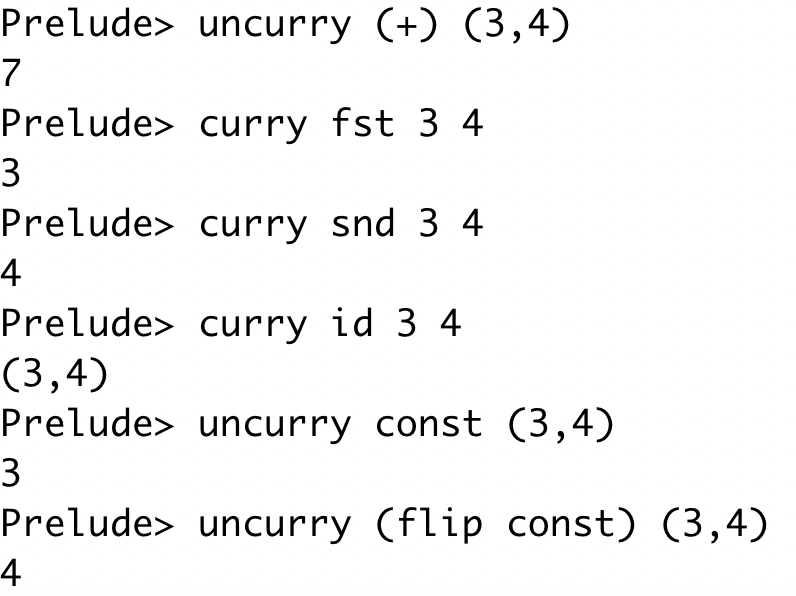
\includegraphics[scale=0.554]{Pics/Curry.png}
  \end{center}
\end{frame}

\begin{frame}[fragile]
  \frametitle{The functions above in the GHCi session. The \verb"flip" example}

  \begin{lstlisting}[language=Haskell]
  show2 :: Int -> Int -> String
  show2 x y = show x ++ " and " ++ show y

  showSnd, showFst, showFst' :: Int -> String
  showSnd  = show2 1
  showFst  = flip show2 2
  showFst' = (`show2` 2)
  \end{lstlisting}

\onslide<2->{
  \begin{center}
  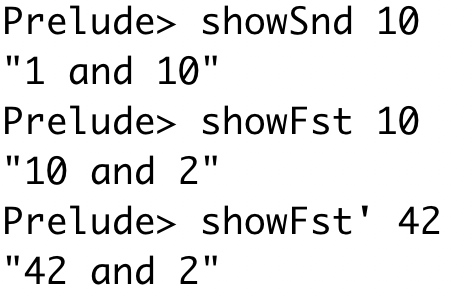
\includegraphics[scale=0.47]{Pics/Flip.png}
  \end{center}
  }
\end{frame}

\begin{frame}[fragile]
  \frametitle{Bye-bye boilerplate!}

  All these functions
  \begin{lstlisting}[language=Haskell]
  changeTwiceBy :: (Int -> Int) -> Int -> Int
  changeTwiceBy operation value = operation (operation value)

  changeTwiceByBool :: (Bool -> Bool) -> Bool -> Bool
  changeTwiceByBool operation value = operation (operation value)

  changeTwiceByString :: (String -> String) -> String -> String
  changeTwiceByString operation value = operation (operation value)
  \end{lstlisting}

  might be replaced to the following ones:
  \begin{lstlisting}[language=Haskell]
  applyTwice :: (a -> a) -> a -> a
  applyTwice f a = f (f a)

  applyTwice' :: (a -> a) -> a -> a
  applyTwice' f a = f . f $ a

  applyTwice'' :: (a -> a) -> a -> a
  applyTwice'' f = f . f
  \end{lstlisting}
\end{frame}

\begin{frame}[fragile]
  \frametitle{HOF, polymorpism, and lists}

  \begin{lstlisting}[language=Haskell]
  map     :: (a -> b)      -> [a] -> [b]

  filter  :: (a -> Bool)   -> [a] -> [a]

  zipWith :: (a -> b -> c) -> [a] -> [b] -> [c]

  length :: [a] -> Int
  \end{lstlisting}

\vspace{\baselineskip}

\onslide<2->{
  We discuss their implementations closely on the next seminar. Here we just take a look at their behaviour.
  }
\end{frame}

\begin{frame}[fragile]
    \frametitle{The composition examples + list functions}
\begin{lstlisting}[language=Haskell]
foo, bar :: [Int] -> Int
foo patak =
  length $ filter odd $
  map (div 2) $ filter even $ map (div 7) patak

bar       =
  length . filter odd .
  map (div 2) . filter even . map (div 7)

zip :: [a] -> [b] -> [(a, b)]
zip = zipWith (,)
\end{lstlisting}
\end{frame}

\begin{frame}[fragile]
    \frametitle{The composition examples + list functions}
    \begin{lstlisting}[language=Haskell]
    stringsTransform :: [String] -> [String]
    stringsTransform l = map (\s -> map toUpper s) (filter (\s -> length s == 5) l)

    stringsTransform l = map (\s -> map toUpper s) $ filter (\s -> length s == 5) l

    stringsTransform l = map (map toUpper) $ filter ((== 5) . length) l

    stringsTransform = map (map toUpper) . filter ((== 5) . length)
    \end{lstlisting}
\end{frame}

\begin{frame}
  \frametitle{Bounded polymorphism and type classes}

\onslide<1->{
  The idea of bounded (ad hoc) polymorphism is that one has a general interface with instances for each concrete data type.
}

\onslide<2->{
\begin{center}
\includegraphics[scale=0.35]{Pics/NineAdHoc.png}
\end{center}
}
\end{frame}

\begin{frame}[fragile]
  \frametitle{Type classes. Motivation}

\begin{itemize}
  \item Let us take a look a the following function

  \begin{lstlisting}[language=Haskell]
  elem :: a -> [a] -> Bool
  elem _ [] = False
  elem x (y:ys) = x == y || elem x ys
  \end{lstlisting}

\onslide<2->{
  \item Is a type \verb"a" arbitrary?} \onslide<3->{Yes and no. \verb"a" is an arbitrary type for which equality is defined.}
\end{itemize}
\end{frame}

\begin{frame}[fragile]
  \frametitle{Type classes. Motivation}
  As we observed, type variables in polymorphic function are bounded via universal quantifier. In ad hoc polymorphism, type variables are also bounded via $\forall$ but with the additional condition. Such a quantification is called bounded.

  \begin{lstlisting}[language=Haskell]
  elem :: forall a. Eq a => a -> [a] -> Bool
  elem _ [] = False
  elem x (y:ys) = x == y || elem x ys
  \end{lstlisting}

\end{frame}

\begin{frame}[fragile]
  \frametitle{The notion of a type class}

\begin{itemize}
  \item \emph{A type class} is a collection of functions with type signatures with a common type parameter. The example given:

  \begin{lstlisting}[language=Haskell]
  class Eq a where
    (==) :: a -> a -> Bool
    (/=) :: a -> a -> Bool
  \end{lstlisting}

  \item A type class name introduce a constraint called \emph{context}:

  \begin{lstlisting}[language=Haskell]
  elem :: Eq a => a -> [a] -> Bool
  elem _ [] = False
  elem x (y:ys) = x == y || elem x ys
  \end{lstlisting}
\onslide<2->{
  \item The definition above without a context yields a type error:
  \begin{center}
  \includegraphics[scale=0.24]{Pics/EqError.png}
  \end{center}
}
\end{itemize}
\end{frame}

\begin{frame}[fragile]
  \frametitle{Instance declarations}

  A given data type \verb"a" has the \emph{instance} of a type class if every function of that class is implemented for \verb"a". The example:

  \begin{lstlisting}[language=Haskell]
  instance Eq Bool where
    True == True   = True
    False == False = True
    _ == _         = False

    x /= y        = neg (x == y)
  \end{lstlisting}
\end{frame}

\begin{frame}[fragile]
  \frametitle{Polymorphism + instance declarations}

\begin{itemize}
  \item A type parameter in an instance declaration might be polymorphic itself:

  \begin{lstlisting}[language=Haskell]
  instance Eq a => Eq [a] where
    []       == []       = True
    (x : xs) == (y : ys) = x == y && xs == ys
    _        == _        = False
  \end{lstlisting}
  \item Without the context \verb"Eq a =>", this definition yields type error since we don't know how to perform
  equality comparison of element from \verb"a"
\end{itemize}
\end{frame}

\begin{frame}[fragile]
  \frametitle{Some the \verb"Eq" instances}

\begin{itemize}
\item The \verb"Eq" type class has the following instances (some of them)

  \begin{lstlisting}[language=Haskell]
  instance Eq a => Eq [a]
  instance Eq Ordering
  instance Eq Int
  instance Eq Float
  instance Eq Double
  instance Eq Char
  instance Eq Bool
  \end{lstlisting}
\item See the standard library source code to take a look at the instances implementation.
\end{itemize}
\end{frame}

\begin{frame}[fragile]
  \frametitle{The \verb"Show" type class}

\begin{itemize}
  \item The \verb"Show" type class allows one to represent a value as a string:
  \begin{lstlisting}[language=Haskell]
  class Show a where
    showsPrec :: Int -> a -> ShowS
    show :: a -> String
    showList :: [a] -> ShowS
    {-# MINIMAL showsPrec | show #-}
  \end{lstlisting}
  \item One needs to have a \verb"Show" instance to display a value of a given type on a console.
\end{itemize}
\end{frame}

\begin{frame}[fragile]
  \frametitle{Some of the \verb"Show" instances}

Here are some of the \verb"Show" instances:
\begin{lstlisting}[language=Haskell]
  instance Show Integer
  instance Show Int
  instance Show Char
  instance Show Bool
  instance (Show a, Show b) => Show (a, b)
\end{lstlisting}
\end{frame}

\begin{frame}[fragile]
  \frametitle{Ordering. Motivation}
  \begin{itemize}
  \item Let us take a look at the following quicksort function:

  \begin{lstlisting}[language=Haskell]
  quicksort :: [a] -> [a]
  quicksort [] = []
  quicksort (x:xs) = quicksort small ++ (x : quicksort large)
    where
      small = [y | y <- xs, y <= x]
      large = [y | y <- xs, y > x]
  \end{lstlisting}
  \onslide<2->{
  \item Here we have the same story as in the case of equality. A type \verb"a" is an arbitrary type for which comparison is defined. The definition of quicksort as above is wrong. There exists a type element of which are incomparable, complex numbers, e.g.
  }
\end{itemize}
\end{frame}

\begin{frame}[fragile]
  \frametitle{The \verb"Ord" type class}

The full definition of \verb"Ord" is the following one:

  \begin{lstlisting}[language=Haskell]
  class Eq a => Ord a where
    compare :: a -> a -> Ordering
    (<), (<=), (>), (>=) :: a -> a -> Bool
    max, min :: a -> a -> a

    compare x y = if x == y then EQ
              else if x <= y then LT
              else GT

    x <= y = case compare x y of { GT -> False; _ -> True }

    max x y = if x <= y then y else x

    {-# MINIMAL compare | (<=) #-}
  \end{lstlisting}
\end{frame}

\begin{frame}[fragile]
  \frametitle{Some of the \verb"Ord" instances}

\begin{itemize}
  \item The \verb"Ord" instances
\begin{lstlisting}[language=Haskell]
  instance Ord Int
  instance Ord Float
  instance Ord Double
  instance Ord Char
  instance Ord Bool
\end{lstlisting}
\end{itemize}
\end{frame}

\begin{frame}[fragile]
  \frametitle{The \verb"Num" type class}

\begin{itemize}
  \item \verb"Num" is a type class with the general interface of usual arithmetical operations.
  \begin{lstlisting}[language=Haskell]
  class Num a where
    (+), (-), (*) :: a -> a -> a
    negate, abs, signum :: a -> a
    fromInteger :: Integer -> a
    {-# MINIMAL (+), (*), abs, signum, fromInteger, (negate | (-)) #-}
  \end{lstlisting}
  \onslide<2->{
  \item The instances of \verb"Num" form a collection of numerical data types in Haskell
  } \onslide<3->{
  \item Note that we don't require the context \verb"Ord a" since the set complex numbers is an instance of \verb"Num", but we don't have the instance \verb"Ord Complex", as you know.
  }
\end{itemize}
\end{frame}

\begin{frame}[fragile]
  \frametitle{Some of the \verb"Num" instances}

\begin{itemize}
\item The examples of \verb"Num" instances are:

\begin{lstlisting}[language=Haskell]
  instance Num Integer
  instance Num Int
  instance Num Float
  instance Num Double
\end{lstlisting}
\end{itemize}
\end{frame}

\begin{frame}[fragile]
  \frametitle{The \verb"Enum" and \verb"Bounded" type classes}

\begin{itemize}
  \item The \verb"Enum" is type class for type for which one may define an explicit enumeration.
\begin{lstlisting}[language=Haskell]
  class Enum a where
    succ, pred :: a -> a
    toEnum     :: Int -> a
    fromEnum   :: a -> Int

    enumFrom       :: a -> [a]            -- [n..]
    enumFromThen   :: a -> a -> [a]       -- [n,m..]
    enumFromTo     :: a -> a -> [a]       -- [n..m]
    enumFromThenTo :: a -> a -> a -> [a]  -- [n,m..p]
    {-# MINIMAL toEnum, fromEnum #-}
  \end{lstlisting}

\item The \verb"Bounded" type class is a type class for bounded types, i.e., types with minimal and maximal bounds
\begin{lstlisting}[language=Haskell]
  class Bounded a where
    minBound :: a
    maxBound :: a
    {-# MINIMAL minBound, maxBound #-}
  \end{lstlisting}
\end{itemize}
\end{frame}

\begin{frame}[fragile]
  \frametitle{Some of the \verb"Enum" instances}

\begin{itemize}
  \item The instances are the following ones:
\begin{lstlisting}[language=Haskell]
  instance Enum Integer
  instance Enum Int
  instance Enum Char
  instance Enum Bool
  instance Enum Float
  instance Enum Double
\end{lstlisting}
\end{itemize}
\end{frame}

\begin{frame}[fragile]
  \frametitle{Some of the \verb"Bounded" instances}
\begin{itemize}
  \item The examples of bounded data types
\begin{lstlisting}[language=Haskell]
  instance Bounded Int
  instance Bounded Char
  instance Bounded Bool
\end{lstlisting}
\end{itemize}
\end{frame}

\begin{frame}[fragile]
  \frametitle{The \verb"Fractional" type class}

\begin{itemize}
  \item The \verb"Fractional" type class is a general interface for numerical division
\begin{lstlisting}[language=Haskell]
  class Num a => Fractional a where
    (/) :: a -> a -> a
    recip :: a -> a
    fromRational :: Rational -> a
    {-# MINIMAL fromRational, (recip | (/)) #-}
  \end{lstlisting}
  \item It is clear that such a type should be a numerical one. Thus, we require the \verb"Num a" restriction.
  \item The \verb"Fractional" instances:
  \begin{lstlisting}[language=Haskell]
  instance Fractional Float
  instance Fractional Double
  \end{lstlisting}
\end{itemize}
\end{frame}

\begin{frame}
  \frametitle{Summary}

\onslide<1->{
  On this seminar, we
  \begin{itemize}
    \item took a look at parametric polymorphism to see how to avoid boilerplate
    \item discussed type classes and ad hoc polymorphism
    \item studied such basic type classes as \verb"Eq", \verb"Show", etc
  \end{itemize}
}

\onslide<2->{
On the next seminar, we
  \begin{itemize}
    \item delve into the variety of Haskell data types: algebraic data types, newtypes,
    type synonyms, etc
    \item feel the power of pattern matching
    \item discuss folds
    \item see how to enforce lazy evaluation in Haskell
  \end{itemize}
}
\end{frame}


\end{document}
